\section{COMSOL implementation}
\label{app:comsol_deriv}

The commercial software COMSOL
allows us to perform thermal simulations
with a finite-element approach.
The heat equation
to be solved
reads as
\begin{equation}
0 = \nabla(k\nabla T) + Q.
\label{eq:app:heateq}
\end{equation}
It is $k$ the thermal conductivity of the material
($[k]=\mathrm{m}^{-1}$),
and $Q$ the heat source
($[Q]=\mathrm{W}/\mathrm{m}^3$);
originating from the pump beam.
Before we can talk about
the numerical insights
found with COMSOL,
we have to understand
the necessary parameters
and their influence
on this model.

\subsection{Heat source $Q$}
\label{app:comsol_deriv:Q}

In order to understand
how to investigate
the temperature distribution
within a VECSEL structure,
we have to understand
what input to provide to COMSOL
to solve the heat equation (\ref{eq:app:heateq}).
Our optical pumping represents
a heat source $Q$.
In this subsection
I present what this quantity looks like,
and what influence the different parameters --
most notably, the beam profile --
have.

The pump beam
is assumed to be
incident antiparallel to the $z$-axis
(here referred to as from the top).
We assume further
it is of Gaussian profile --
section~\ref{sec:comsol:beamprofile}
explains how to incorporate
different pump profiles.
In this configuration the heat source
associated with
each layer $j$ of the structure is given as
\cite{Kemp2008}
\begin{equation}
Q_j = \frac{2P}{\pi w^2} \eta_j\alpha_j \e^\frac{-2r^2}{w^2} \e^{-\alpha_j(z_{0j}-z)} \e^{-\sum_{i<j}\alpha_i t_i}.
\label{eq:app:heatsrc}
\end{equation}
The layers are counted from the top down --
the sum $\sum_{i<j}$ includes the layers on top
and ignores those below the layer of interest
(in that case $j$).
The meaning of the single parameters are listed in Tab.~\ref{tab:heatsrc}.
Furthermore we recognize
\begin{equation}
P'=P\e^{-\sum_{i<j}\alpha_i t_i}
\end{equation}
to represent the power still remaining after layer $1,2,\ldots,j$.
And
\begin{equation}
A=P'\eta_j
\end{equation}
corresponds
to the absorbed power in layer $j$;
which heats by factor $\alpha_j$.

\begin{table}[h]
\centering
\caption{Meaning of parameters used in (\ref{eq:app:heatsrc}).}
\begin{tabular}{llc}
\hline
Parameter & Explanation & Unit \\
\hline
$P$ & pump power & $\mathrm{W}$ \\
$w$ & pump beam $1/e^2$ radius & $\mathrm{m}$ \\
$\alpha_j$ & absorption coefficient of layer $j$ & $\mathrm{m}^{-1}$ \\
$r$ & radial coordinate & $\mathrm{m}$ \\
$z$ & axial coordinate & $\mathrm{m}$ \\
$z_{0j}$ & coordinate of top of layer $j$ & $\mathrm{m}$ \\
$t_j$ & thickness of layer $j$ & $\mathrm{m}$ \\
$\eta_j$ & heat loading fraction in layer $j$ & - \\
\hline
\end{tabular}
\label{tab:heatsrc}
\end{table}

The Gaussian beam assumed in (\ref{eq:app:heatsrc})
has an E-field \cite{QE}
\begin{equation}
E(r,z) \propto \frac{w_0}{w(z)} \exp(-\frac{r^2}{w^2(z)}) \exp(-i\Phi).
\label{eq:gaussE}
\end{equation}
The intensity of such a beam is proportional to the square modulus
\begin{align}
I(r,z) &\propto |E(r,z)|^2, \\
I(r,z) &= I_0 \left(\frac{w_0}{w(z)}\right)^2 \exp(-\frac{2r^2}{w^2(z)}).
\label{eq:gaussI}
\end{align}
This is where the factor $2$
in the exponent of (\ref{eq:app:heatsrc})
comes from.
The over all power
contained within the cross section
is constant, $P$.
Hence follows
the last part of (\ref{eq:app:heatsrc})
\begin{align}
P &= \int\limits_0^{2\pi}\d\varphi\int\limits_0^\infty r\d r I(r,z) \\
 &= 2\pi I_0 \left(\frac{w_0}{w(z)}\right)^2 \int\limits_0^\infty r \d r \exp(-\frac{2r^2}{w^2(z)}) \\
 &= 2\pi I_0 \left( \frac{w_0}{w(z)}\right)^2 \left[ -\frac{w^2(z)}{4} \exp(-\frac{2r^2}{w^2(z)}) \right]_0^\infty \\
 &= \frac{\pi}{2} w_0^2 I_0, \\
\Rightarrow\quad I_0 &= \frac{2P}{\pi w_0^2}.
\end{align}

\subsection{Implementation of our VECSEL structure}
\label{app:comsol_deriv:impl}

In this subsection I discuss the parameters
relevant for the actual COMSOL implementation,
taking our structure as an example
\cite{Ranta2014OptLett}.
A schematic of our VECSEL structure
is depicted in Fig.~\ref{img:design}.
Its fabrication details can be found in
\cite{Ranta2014OptLett,Sirbu2014SPIE}.
A summary of the used parameters --
in order to reproduce the presented results --
is given in appendix~\ref{app:comsolparams},
Tab.~\ref{tab:comsolparams}.

For the thermal conductivity
we have to consider
its spatial anisotropy.
The radial and axial thermal conductivity
we find with
\cite{Vetter2012,Lindberg2005,Osinski1993}
\begin{align}
k_r &= \frac{\sum_i k_i t_i}{\sum_i t_i} \\
k_z &= \frac{\sum_i t_i}{\sum_i \frac{t_i}{k_i}},
\label{eq:radaxthermcond}
\end{align}
with the actual values calculated from \cite{ioffe}
\begin{equation}
k_{\mathrm{Al}_{x}\mathrm{Ga}_{1-x}\mathrm{As}} =
0.55-2.12x+2.48x^2\,\mathrm{Wcm}^{-1}\mathrm{K}^{-1}.
\label{eq:k_AlGaAs}
\end{equation}
Before we employ
the extracted values of
a bulk Al$_{x}$Ga$_{1-x}$As material,
we divide them in half.
This way we account for
the empirically observed decrease
in thermal conductivity
in a layered structure such as a DBR
\cite{Piprek1998,Ranta2014APL}.

The absorption coefficient $\alpha_\mathrm{g}$ 
is chosen such that
it matches with the measured single pass absorption of $50\,\%$
\cite{Ranta2014OptLett}:
\begin{equation*}
\e^{-\alpha_\mathrm{g}t_\mathrm{g}}=0.5.
\end{equation*}

As a last important note we have to account
for the reflected beam:
it is absorbed in the gain section once again.
Hence we implement a second heat source in this gain layer
according to (\ref{eq:heatsrc})
\begin{equation}
Q_{\mathrm{g}_\mathrm{refl}} = \frac{2P}{\pi w^2} \eta_{\mathrm{g}_\mathrm{refl}}\alpha_g \e^\frac{-2r^2}{w^2} \e^{-\alpha_g(z_{0g}-t_g+z)}
 \e^{-\alpha_\mathrm{InP} t_c -\alpha_\mathrm{g} t_\mathrm{g} -2\alpha_\mathrm{InP}t_\mathrm{sp} -2\alpha_\mathrm{d}t_\mathrm{d}}.
\label{eq:heatsrcrefl}
\end{equation}
In this we have the expression
\begin{equation}
\eta_{\mathrm{g}_\mathrm{refl}} = \eta_\mathrm{g} (1-\eta_\mathrm{au}),
\label{eq:etagrefl}
\end{equation}
that assumes the fraction of reflected light
to be the residual light of what was not absorbed by the gold layer.
This remaining part heats the layer with efficiency $\eta_\mathrm{g}$.
Furthermore we see the sign in the exponent
\begin{equation*}
\e^{-\alpha_g(z_{0g}-t_g+z)}
\end{equation*}
to be positive.
This comes from the fact that in reflection
the beam travels in the opposite direction.

\subsection{Numeric convergence based on dimensionality}
\label{app:numconv}

\begin{figure}
\centering
\subfigure{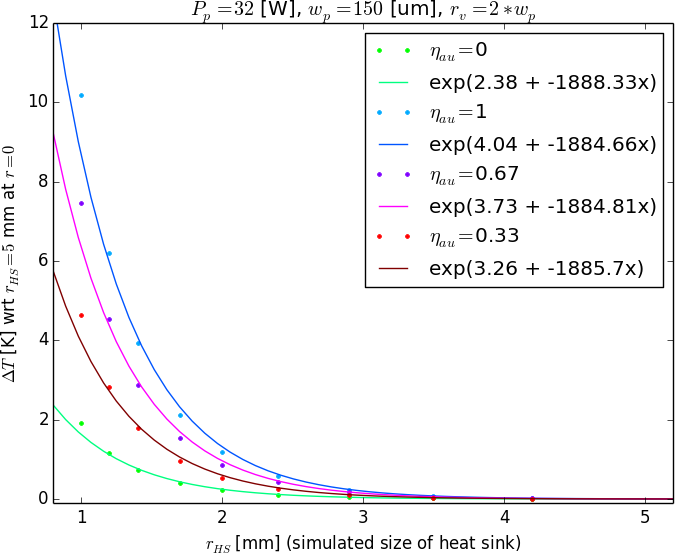
\includegraphics[width=7cm]{img/appendix/r_HS-vs-T.png}}
\subfigure{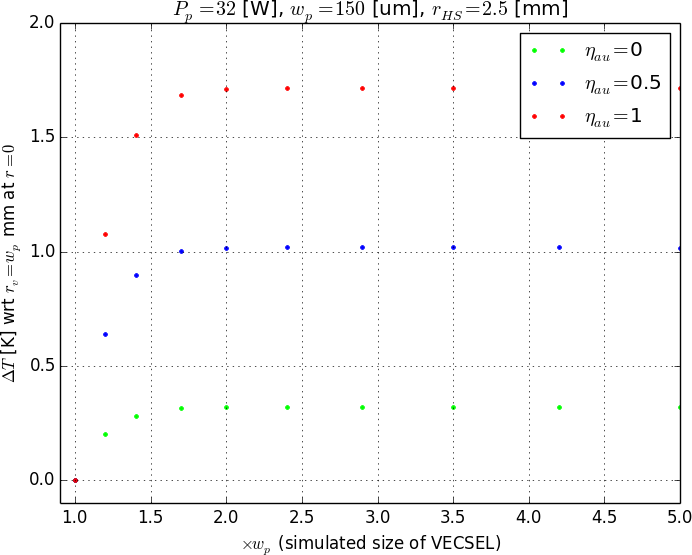
\includegraphics[width=7cm]{img/appendix/r_v-vs-T.png}}
\caption{Left: Investigating on the convergence of the result,
depending on the system's dimension.
The size considered for the heat sink
is exponentially important.
Right: Investigating on the convergence of the result,
depending on the dimension of the VECSEL.
Considering a system larger than $2w_\mathrm{p}$
doesn't influence the over all result.}
\label{img:r_HS-r_v-vs-dT}
\end{figure}

Measuring the performance of a sample
in an experiment
is not the same as simulating it
numerically.
With COMSOL we can exploit
certain symmetries
imposed by the structure.
One is the radial symmetry
around an irradiated spot,
so that COMSOL has to solve
the equations only in two
rather than three dimensions --
which speeds up the calculations.
A second common simplification
is to simulate the VECSEL dimensions
only up to twice the size
of the pump spot \cite{Kemp2008}.
In order to ensure
such simplifications
don't lead to wrong conclusions,
we have to investigate
on the convergence behavior
depending on these parameters.
The names of parameters
are taken from
appendix~\ref{app:comsol_deriv:Q}--\ref{app:comsol_deriv:impl}
and Tab.~\ref{tab:comsolparams}.

Figure~\ref{img:r_HS-r_v-vs-dT} (left) presents
the convergence of the numerical result
depending on the system's size.
Each data point represents the following:
I simulate the temperature
on the surface of the structure
caused by a $P=32\,\mathrm{W}$,
$2w_p=300\,\mu\mathrm{m}$ pump diameter beam.
The radius of the VECSEL
is held constant at
$r_\mathrm{v}=2w_\mathrm{p}$.
In the center (at $r=0$)
the temperature is the highest;
this is the value we store,
for each system size $r_\mathrm{HS}$;
the considered radius of the heat sink.
For different values of $\eta_\mathrm{au}$
I look at various radii between
$r_\mathrm{HS}=1\,\mathrm{mm}$
and $r_\mathrm{HS}=5\,\mathrm{mm}$
(twice the size of our actual structure
with a cross section of $5\times5\,\mathrm{mm}^2$).
In the plot $\Delta T$ refers to the difference
between the temperature obtained with
the $r_\mathrm{HS}$ specified along the x-axis
and the temperature with $r_\mathrm{HS}=5\,\mathrm{mm}$.

The larger $r_\mathrm{HS}$ is chosen,
the less relevant is its actual value --
the temperature spread due to the extra bulk material
goes exponentially.
Therefore,
it seems to be important
to simulate the heat sink
(diamond layer and copper bulk)
as its full size.
The size of the VECSEL on the other hand
seems to be far less important;
its over all volume
and thus its ability to store and transfer heat
is small.
VESCEL sizes larger than two times the beam radius
result in the same temperature increase.
This statement is visualized
in Fig.~\ref{img:r_HS-r_v-vs-dT} (right).
In this plot,
the heat sink is kept
at constant $r_\mathrm{HS}=2.5\,\mathrm{mm}$ and
$r_\mathrm{v}$ is varied as multiples of $w_\mathrm{p}$.

The influence of the considered thickness of the gold layer
depends on whether or not
the incident beam is absorbed in this interface --
i.e. whether the gold layer only conducts the heat,
or is itself a heat source.
Figure~\ref{img:t_au-t_HS-vs-dT} (left)
illustrates this consideration.

\begin{figure}
\centering
\subfigure{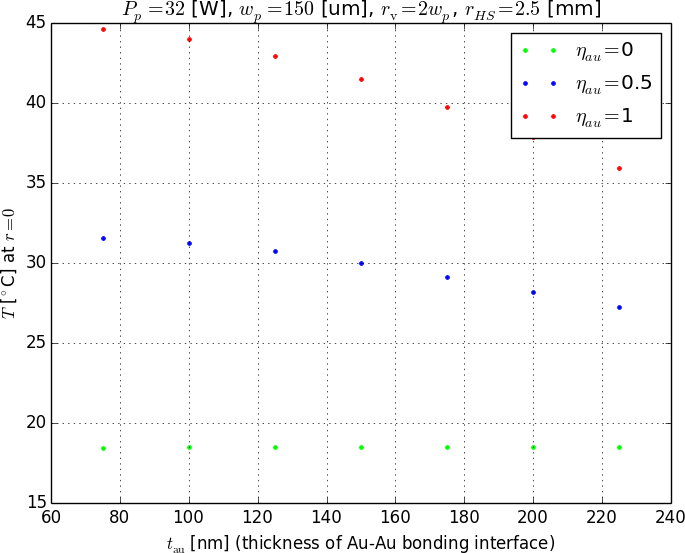
\includegraphics[width=7cm]{img/appendix/t_au-vs-T.png}}
\subfigure{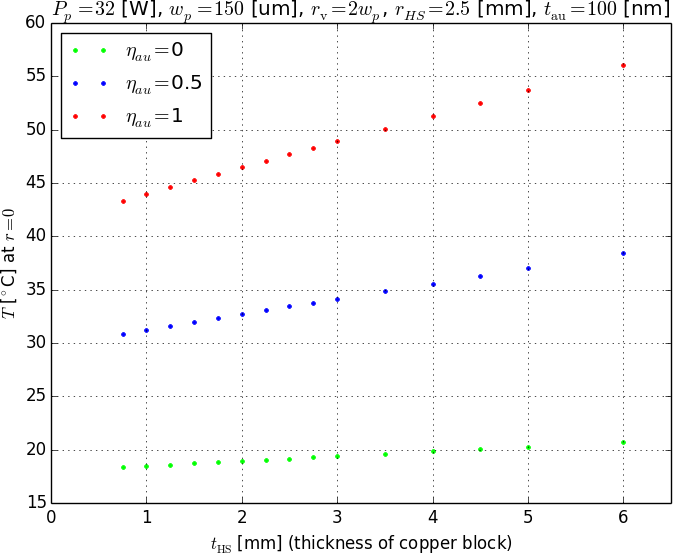
\includegraphics[width=7cm]{img/appendix/t_HS-vs-T.png}}
\caption{Left: Investigating on the convergence of the result,
depending on the thickness of the Au-Au bonding interface.
If we assume the gold layer
absorbs at least some of the incident beam,
we have to know the thickness of this layer.
Right: Investigating on the convergence of the result,
depending on the thickness of the copper heat sink considered.
Its importance depends on whether or not
we assume the gold layer to act as a heat source.}
\label{img:t_au-t_HS-vs-dT}
\end{figure}

In order to look at the influence of
the heat sink copper block
we assume
$r_\mathrm{HS}=2.5\,\mathrm{mm}$,
$r_\mathrm{v}=2w_\mathrm{p}$,
$t_\mathrm{au}=100\,\mathrm{nm}$.
The bottom boundary of the copper block
is held at constant temperature.
A thicker copper heat sink hence means
that the heat has to travel a longer distance.
As shown in Fig.~\ref{img:t_au-t_HS-vs-dT} (right)
this extra distance is relevant;
especially if we consider the gold layer
to act as a heat source.


\subsection{Explicit listing of simulation parameters}
\label{app:comsolparams}

Because numerical simulations are difficult to reproduce
when the used parameters are unknown,
the ones I used for section~\ref{sec:comsol}
are listed in Tab.~\ref{tab:comsolparams}.

\begin{table}[h]
\centering
\caption{Parameters used in the COMSOL simulation
reported in section~\ref{sec:comsol}.}
\begin{tabular}{lll}
\hline
 & Quantity & Value \\
\hline
$P_\mathrm{p}$ & Pump power & $32\,\mathrm{W}$ \\
$w_\mathrm{p}$ & Pump beam radius ($1/\e^2$) & $100\,\mathrm{\mu m}$ \\
$t_\mathrm{c}$ & Thickness cap [Specs] & $0.1017\,\mathrm{\mu m}$ \\
$t_\mathrm{g}$ & Thick. gain [Specs] & $0.7785\,\mathrm{\mu m}$ \\
$t_\mathrm{sp}$ & Thick. InP spacer [$\lambda$, Specs] & $0.4039\,\mathrm{\mu m}$ \\
$t_\mathrm{d}$ & Thick. DBR [Specs] & $5.0709\,\mathrm{\mu m}$ \\
$t_\mathrm{au}$ & Thick. Au layer [estimate] & $200\,\mathrm{nm}$ \\
$t_\mathrm{dia}$ & Thick. diamond layer & $0.3\,\mathrm{mm}$ \\
$t_\mathrm{HS}$ & Thick. copper heat sink & $3\,\mathrm{mm}$ \\
$k_\mathrm{InP}$ & Thermal conductivity InP \cite{Piprek2002} & $68\,\mathrm{W/(K\cdot m)}$ \\
$k_\mathrm{g}$ & Therm. cond. gain \cite{Piprek2002} & $4\,\mathrm{W/(K\cdot m)}$ \\
$k_\mathrm{d}$ & Therm. cond. DBR \cite{Piprek1998} & $0.35\,\mathrm{W/(cm\cdot K)}$ \\
$k_\mathrm{dr}$ & Therm. cond DBR in radial \cite{Vetter2012,ioffe,Piprek1998} & $36.8\,\mathrm{W/(m\cdot K)}$ \\
$k_\mathrm{dz}$ & Therm. cond DBR in z \cite{Vetter2012,ioffe,Piprek1998} & $34.6\,\mathrm{W/(m\cdot K)}$ \\
$k_\mathrm{dia}$ & Therm. cond. diamond \cite{Ranta2014OptLett} & $1800\,\mathrm{W/(m\cdot K)}$ \\
$k_\mathrm{au}$ & Therm. cond of gold \cite{SpringerMat} & $320\,\mathrm{W/(m\cdot K)}$ \\
$\alpha_\mathrm{InP}$ & Absorption coeff InP at 980 nm \cite{SpringerMat,ioffe} & $0\,\mathrm{mm}^{-1}\mathrm{}$ \\
$\alpha_\mathrm{g}$ & Absorpt. gain \cite{Ranta2014OptLett} & $0.9\times 10^{6}\,\mathrm{m}^{-1}\mathrm{}$ \\
$\alpha_\mathrm{d}$ & Abs. DBR at 980 nm \cite{SpringerMat,ioffe} & $0\,\mathrm{mm}^{-1}\mathrm{}$ \\
$\alpha_\mathrm{au}$ & Abs. Au \cite{SpringerMat,ioffe,Schubert} & $86554\,\mathrm{mm}^{-1}\mathrm{}$ \\
$\lambda_\mathrm{p}$ & Pump wavelength & $980\,\mathrm{nm}$ \\
$\lambda_\mathrm{L}$ & Laser wavelength & $1270\,\mathrm{nm}$ \\
$\eta_\mathrm{c}$ & Heat loading fraction: cap & $0$ \\
$\eta_\mathrm{g}$ & Heat loading fraction: gain & $1-\lambda_\mathrm{p}/\lambda_\mathrm{L}$ \\
$\eta_\mathrm{sp}$ & Heat loading fraction: spacer & $0$ \\
$\eta_\mathrm{d}$ & Heat loading fraction: DBR & $0$ \\
$\eta_\mathrm{au}$ & Heat loading fraction: Au & $0.75$ \\
$\eta_\mathrm{g_{refl}}$ & Heat load. frac.: Gain from reflected beam & $\eta_\mathrm{g}*(1-\eta_\mathrm{au})$ \\
$z_\mathrm{0c}$ & Coordinate top of cap & $z_\mathrm{0g}+t_\mathrm{c}$ \\
$z_\mathrm{0g}$ & Coord top of gain & $z_\mathrm{0sp}+t_\mathrm{g}$ \\
$z_\mathrm{0sp}$ & Coord top of spacer & $z_\mathrm{0d}+t_\mathrm{sp}$ \\
$z_\mathrm{0d}$ & Coord top of DBR & $z_\mathrm{0au}+t_\mathrm{d}$ \\
$z_\mathrm{0au}$ & Coord top Au layer; Interf. Au-DBR to be at 0. & $0\,\mathrm{m}$ \\
$z_\mathrm{dia}$ & Coord bottom diamon layer & $z_\mathrm{0au}-t_\mathrm{au}-t_\mathrm{dia}$ \\
$z_\mathrm{HS}$ & Coord bottom HS & $z_\mathrm{dia}-t_\mathrm{HS}$ \\
$r_\mathrm{v}$ & Width of VECSEL; small for better numeric & $2*w_\mathrm{p}$ \\
$r_\mathrm{HS}$ & Width of heat sink (and diamond) & $2.5\,\mathrm{mm}$ \\
$T_\mathrm{C}$ & \degr{0} & $273.16\,\mathrm{K}$ \\
$T_\mathrm{0}$ & Base temperature & $T_C+15\,\mathrm{K}$ \\
$\beta$ & Exponent of Supergaussian & $\{3,4\}$ \\
$a_\beta$ & normalization super-Gaussian & $\{0.5687,0.6267\}$ \\
\hline
\end{tabular}
\label{tab:comsolparams}
\end{table}
